\chapter{Revisão da Literatura}
Começaremos pela definição de um espaço vetorial e seu subespaço, pois, podemos tratar como vetor ao designar um elemento do espaço vetorial de um número $\mathbb{R}$ definido abaixo:

\noindent\textbf{Definição 01:} Seja um conjunto V, não vazio, com duas operações: soma, $V \times V \rightarrow V$, e multiplicação por escalar, $R \times V \rightarrow V$, tais que, para quaisquer $u, v, w \in \mathbb{R}$, satisfaçam as propriedades:
\begin{enumerate}
	\item $(u + v) + w = u + (v + w)$ e $1u = u$.
	\item $u + v = v + u$.
	\item $\exists 0 \in V$ tal que $u + 0 = u$.
	\item $\exists -u \in V$ tal que $u + (-u) = 0$.
	\item $a(u + v) = au + av$.
	\item $(a + b)v = av + bv$.
	\item $(ab)v = a(bv)$.
	\item $1u = u$.
\end{enumerate}

\noindent\textbf{Observação:} $\textbf{0}$ é o vetor nulo.

\noindent\textbf{Observação:} Limitaremos nossa discussão, demonstrações e aplicações dentro do conjuntos dos números reais apenas.

\noindent\textbf{Exemplo 01:} Suponhamos uma matriz $M_{(2, 2)}$, onde é denotado por $M_{(m,n)}$, dado por 
$M = [a_{ij}]_{m \times n}$ podendo ser interpretada dessa forma, $V = M(2, 2)$, onde $V$, é um conjunto não vazio, seus escalares pertencentes ao conjunto dos $\mathbb{R}$, que satisfazem todas as propriedades de um espaço vetorial.

\begin{figure}[H]
	\centering
	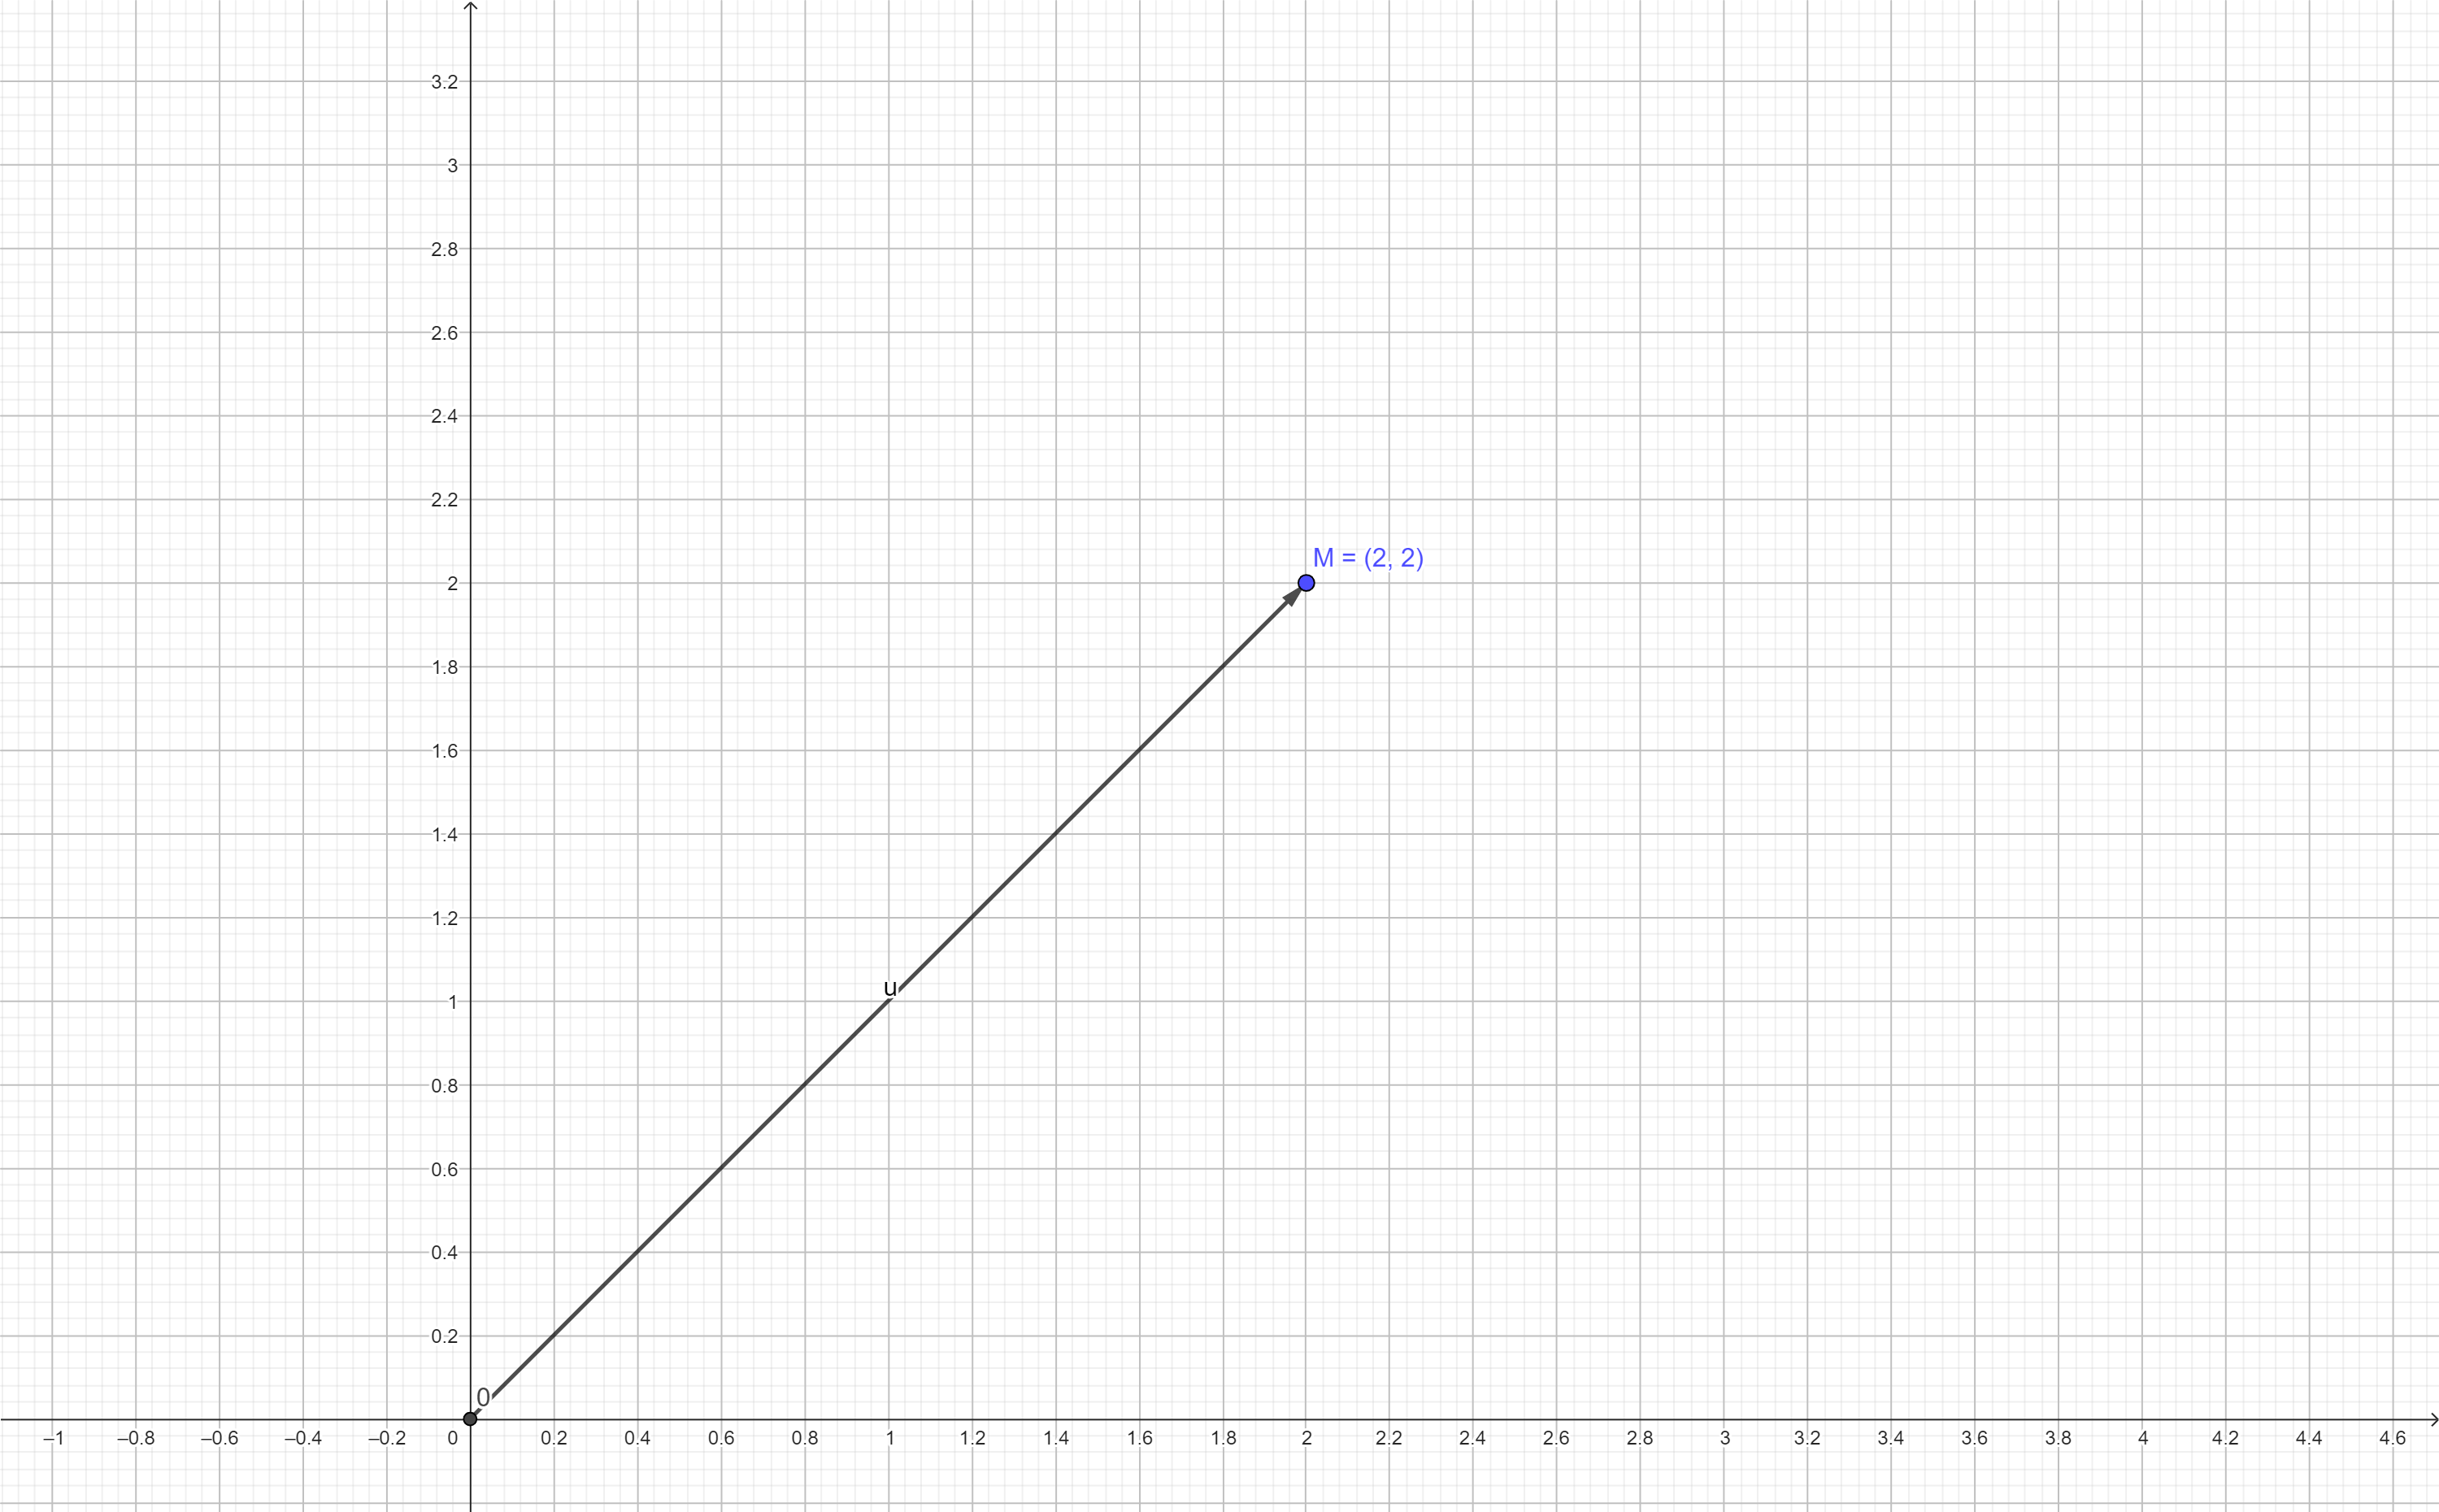
\includegraphics[scale=1.0]{exemplo01.png}
	\caption{Exemplo 01}
\end{figure}

A partir disso, podemos perceber o uso analítico dos espaços vetoriais para resolução de problemas em geral. Vejamos mais alguns exemplos.

\noindent\textbf{Exemplo 02:} O exemplo anterior, tratou-se de plotar uma matriz de $\mathbb{R}^2$ no plano, agora iremos expandir para $\mathbb{R}^3$, seja um vetor $A = (x, y, z)$ ou representado pela forma matricial:

\[
A = \begin{bmatrix}
	a \\ b \\ c
\end{bmatrix}
\]
\noindent Assim, por quaisquer números reais, podemos fazer uma projeção ortogonal no espaço, segue um exemplo traçado:

\begin{figure}[H]
	\centering
	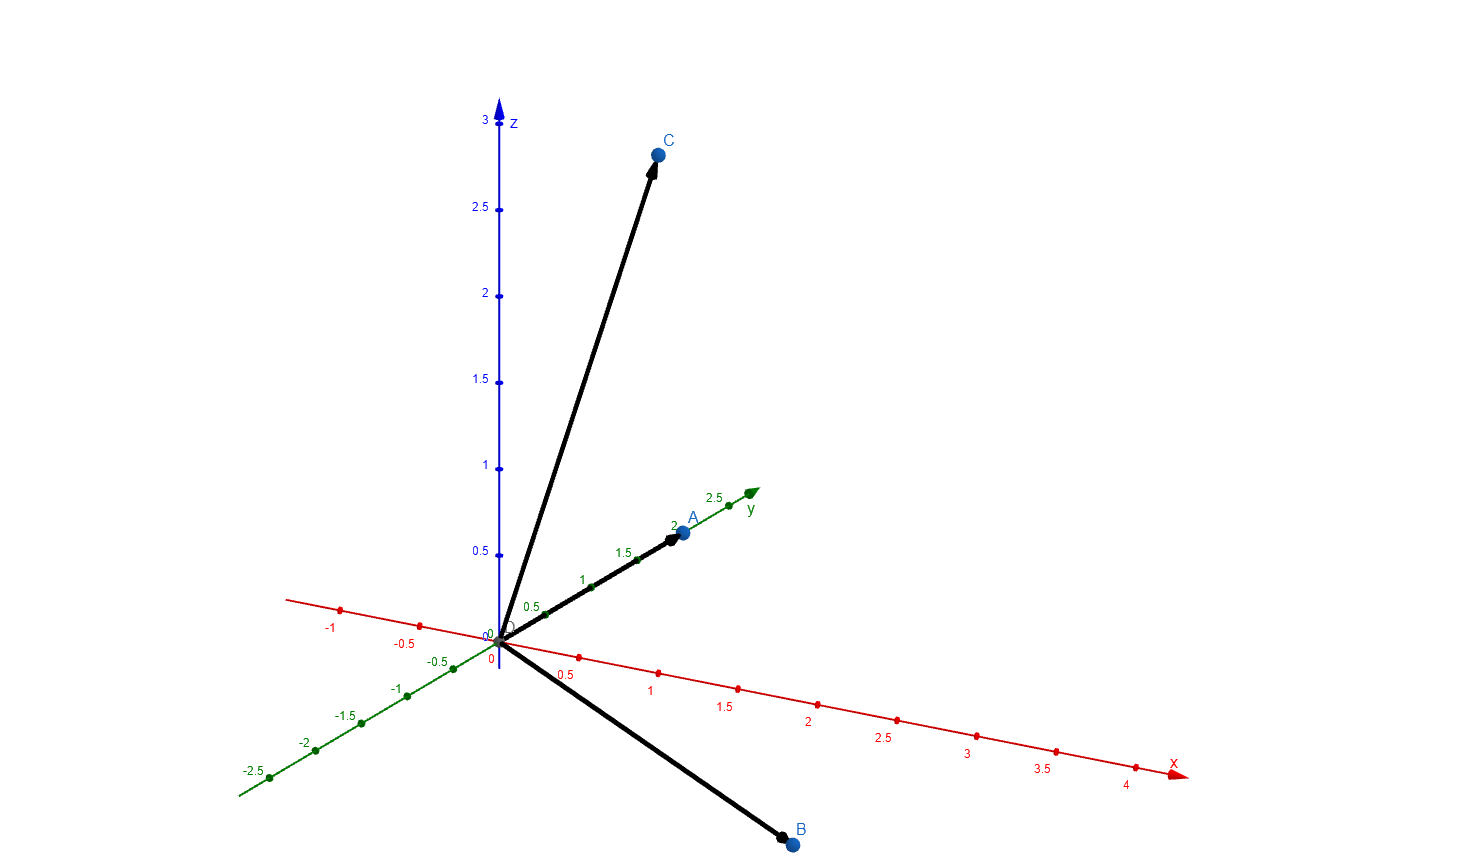
\includegraphics[scale=0.30]{exemplo02.png}
	\caption{Exemplo 02: Exemplo de vetor no espaço.}
\end{figure}

\noindent\textbf{Definição 02:} Dado um espaço vetorial V, um subconjunto W, não vazio, será um subespaço vetorial de V se:
\begin{enumerate}
	\item Para quaisquer $u, v \in W$ tivermos $u + v \in W$.
	\item Para quaisquer $a \in R, u \in W$ tivermos $au \in W$.
	\end{enumerate}

% _{m \times n}

% subinscrito
% _
% expoente com mais de um dígito
% x^{21}
Sabendo tais definições, podemos expressar agora a definição de um transformação linear:

\noindent\textbf{Definição 03:} Sejam V e W dois espaços vetoriais. Uma transformação linear (aplicação linear) é uma função de V em W, $F:V \rightarrow W$, que satisfaz as seguintes condições:
\begin{enumerate}
	\item Para quaisquer $u$ e $v$ em $V$, $F(u + v) = F(u) + F(v)$.
	\item Para quaisquer $k \in R$ e $v \in V$, $F(kv) = kF(v)$.
\end{enumerate}	

